\documentclass[a4paper,12pt,twocolumn]{article}

\usepackage[landscape,top=1cm,bottom=1.4cm,left=1cm,right=1cm,columnsep=1cm]{geometry}
\usepackage[fleqn]{amsmath}
\usepackage{amssymb}
\usepackage{fontspec}
\usepackage{enumitem}
\usepackage{xeCJK}
\usepackage[hidelinks]{hyperref}
\usepackage{tikz}
\usepackage{pgfplots}
\usepgfplotslibrary{groupplots}

\setlength{\mathindent}{1.5em}
\pgfplotsset{compat=1.18}

% Set fonts
\setmainfont{Times New Roman}
\setsansfont{Arial}
\setmonofont{JetBrains Mono}

% Chinese font support
\setCJKmainfont{Iansui}[
  BoldFont=Iansui,
  AutoFakeBold=3.17
]

\pagestyle{plain}
\setlength{\columnseprule}{0.2pt}

\newcommand{\examdate}{2026/04/22}
\newlength{\problemnumberwidth}
\settowidth{\problemnumberwidth}{\textbf{78.}\ }
\newcommand{\problemtitle}[2]{%
  \hypertarget{#1}{}%
  \par\vspace{0.4em}%
  \noindent{\large\bfseries #2}\par
  \vspace{0.3em}%
  \hrule
  \vspace{0.9em}%
}
\newcommand{\worksheettoc}{%
  \noindent{\Large\bfseries Contents}\par
  \vspace{0.3em}%
  \hrule
  \vspace{0.9em}%
  \begin{tabular}{@{}p{0.26\columnwidth}p{0.66\columnwidth}@{}}
    \hyperlink{sec:14-1}{\textbf{14-1}} & \hyperlink{sec:14-1}{32, 48, 49, 52, 56, 78} \\
    \hyperlink{sec:14-2}{\textbf{14-2}} & \hyperlink{sec:14-2}{23, 24, 30, 42, 48, 49} \\
  \end{tabular}\par
}
\newcommand{\problem}[2]{%
  \par\noindent
  \hangindent=\problemnumberwidth
  \hangafter=1
  \makebox[\problemnumberwidth][l]{\textbf{#1.}}#2\par
  \vspace{1.4em}%
}
\newcommand{\problemlead}[2]{%
  \par\noindent
  \hangindent=\problemnumberwidth
  \hangafter=1
  \makebox[\problemnumberwidth][l]{\textbf{#1.}}#2\par
}
\newlist{subparts}{enumerate}{1}
\setlist[subparts]{%
  label = (\alph*),
  labelindent=\problemnumberwidth,
  leftmargin=*,
  labelsep=0.5em,
  align=left,
  itemsep=0.2em,
  topsep=0.3em,
  parsep=0pt,
  partopsep=0pt
}

\pgfplotsset{
  worksheet surface/.style={
    width=3.45cm,
    height=2.85cm,
    xmin=-2.25,
    xmax=2.25,
    ymin=-2.25,
    ymax=2.25,
    domain=-2.25:2.25,
    y domain=-2.25:2.25,
    samples=9,
    samples y=9,
    ticks=none,
    axis lines=none,
    title style={font=\bfseries\large},
    scale only axis,
    clip=false,
    z buffer=sort,
    unbounded coords=jump
  },
  worksheet floor/.style={
    mesh,
    samples=7,
    samples y=7,
    draw=black!22,
    opacity=0.8
  },
  worksheet colored surface/.style={
    surf,
    samples=11,
    samples y=11,
    point meta/expr={0.55*x + 0.35*y + 1.10*z},
    shader=interp,
    fill opacity=0.52,
    draw=none,
    colormap={worksheetpos}{
      color (0cm) = (cyan!35!white);
      color (0.35cm) = (blue!70!cyan);
      color (0.7cm) = (magenta!75!blue);
      color (1cm) = (yellow!70!magenta)
    }
  },
  worksheet axis/.style={
    ->,
    black,
    line width=0.35pt
  }
}

\newcommand{\surfaceaxes}[2]{%
  \addplot3[worksheet floor] {#1};
  \addplot3[worksheet axis] coordinates {(-2.2,0,#1) (2.45,0,#1)}
    node[pos=1, anchor=west, font=\tiny] {$x$};
  \addplot3[worksheet axis] coordinates {(0,-2.2,#1) (0,2.45,#1)}
    node[pos=1, anchor=south west, font=\tiny] {$y$};
  \addplot3[worksheet axis] coordinates {(0,0,#1) (0,0,#2)}
    node[pos=1, anchor=south, font=\tiny] {$z$};
}

\newcommand{\matchgraphsfigure}{%
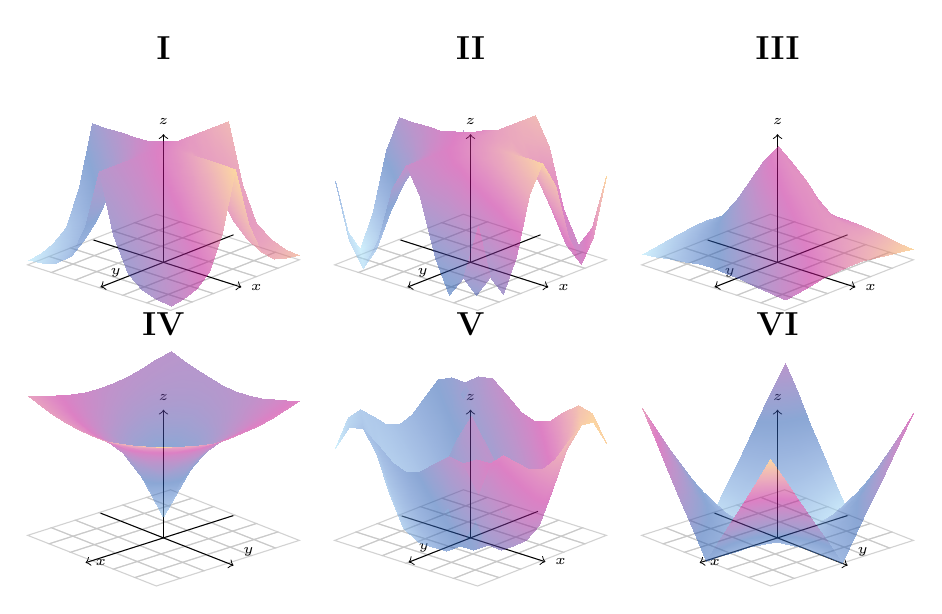
\begin{tikzpicture}
  \begin{groupplot}[
    group style={group size=3 by 2, horizontal sep=0.45cm, vertical sep=0.65cm}
  ]

    \nextgroupplot[
      worksheet surface,
      title={I},
      view={42}{28},
      zmin=0,
      zmax=1.1
    ]
    \surfaceaxes{0}{1.1}
    \addplot3[worksheet colored surface] {1/(1 + x^2*y^2)};

    \nextgroupplot[
      worksheet surface,
      title={II},
      view={42}{28},
      zmin=-1.1,
      zmax=1.1
    ]
    \surfaceaxes{-1.1}{1.1}
    \addplot3[worksheet colored surface] {cos(deg(x*y))};

    \nextgroupplot[
      worksheet surface,
      title={III},
      view={42}{28},
      zmin=0,
      zmax=1.1
    ]
    \surfaceaxes{0}{1.1}
    \addplot3[worksheet colored surface] {1/(1 + x^2 + y^2)};

    \nextgroupplot[
      worksheet surface,
      title={IV},
      view={138}{28},
      zmin=-4.2,
      zmax=1.8
    ]
    \surfaceaxes{-4.2}{1.8}
    \addplot3[worksheet colored surface] {ln(max(x^2 + y^2, 0.04))};

    \nextgroupplot[
      worksheet surface,
      title={V},
      view={42}{28},
      xmin=-5.2,
      xmax=5.2,
      ymin=-5.2,
      ymax=5.2,
      domain=-5.2:5.2,
      y domain=-5.2:5.2,
      zmin=-1.1,
      zmax=1.1
    ]
    \addplot3[worksheet floor, domain=-5.2:5.2, y domain=-5.2:5.2] {-1.1};
    \addplot3[worksheet axis] coordinates {(-5.0,0,-1.1) (5.45,0,-1.1)}
      node[pos=1, anchor=west, font=\tiny] {$x$};
    \addplot3[worksheet axis] coordinates {(0,-5.0,-1.1) (0,5.45,-1.1)}
      node[pos=1, anchor=south west, font=\tiny] {$y$};
    \addplot3[worksheet axis] coordinates {(0,0,-1.1) (0,0,1.1)}
      node[pos=1, anchor=south, font=\tiny] {$z$};
    \addplot3[worksheet colored surface, samples=11, samples y=11]
      {cos(deg(sqrt(x^2 + y^2)))};

    \nextgroupplot[
      worksheet surface,
      title={VI},
      view={138}{28},
      zmin=0,
      zmax=5.1
    ]
    \surfaceaxes{0}{5.1}
    \addplot3[worksheet colored surface] {abs(x*y)};
  \end{groupplot}
\end{tikzpicture}%
}

\begin{document}

\twocolumn[
{\centering
\Large\bfseries Calculus Problems\par
\vspace{0.5em}
\noindent\hfill\normalsize\normalfont \examdate\par
\vspace{0.8em}
}
]

\worksheettoc
\vfill\null
\newpage

\problemtitle{sec:14-1}{14-1}

\problemlead{32}{Match the function with its graph (labeled I--VI). Give reasons for your choices.
\[
\begin{alignedat}{2}
(a)\quad & f(x,y)=\frac{1}{1+x^2+y^2} \qquad &
(b)\quad & f(x,y)=\frac{1}{1+x^2y^2} \\
(c)\quad & f(x,y)=\ln(x^2+y^2) \qquad &
(d)\quad & f(x,y)=\cos \sqrt{x^2+y^2} \\
(e)\quad & f(x,y)=|xy| \qquad &
(f)\quad & f(x,y)=\cos(xy)
\end{alignedat}
\]}
\begin{center}
\matchgraphsfigure
\end{center}
\vspace{1.4em}

\problem{48}{Draw a contour map of the function showing several level curves.
\[
f(x,y)=\ln(x^2+4y^2)
\]}

\problem{49}{Draw a contour map of the function showing several level curves.
\[
f(x,y)=ye^x
\]}

\problem{52}{Draw a contour map of the function showing several level curves.
\[
f(x,y)=\frac{y}{x^2+y^2}
\]}

\problem{56}{If \(V(x,y)\) is the electric potential at a point \((x,y)\) in the \(xy\)-plane, then the level curves of \(V\) are called equipotential curves because at all points on such a curve the electric potential is the same. Sketch some equipotential curves if
\[
V(x,y)=\frac{c}{\sqrt{r^2-x^2-y^2}},
\]
where \(c\) is a positive constant.}

\problem{78}{Investigate the family of surfaces
\[
z=(ax^2+by^2)e^{-x^2-y^2}
\]
How does the shape of the graph depend on the numbers \(a\) and \(b\)?}

\problemtitle{sec:14-2}{14-2}

\problem{23}{Find the limit, if it exists, or show that the limit does not exist.
\[
\lim_{(x,y)\to(0,0)} \frac{xy^2\cos y}{x^2+y^4}
\]}

\problem{24}{Find the limit, if it exists, or show that the limit does not exist.
\[
\lim_{(x,y)\to(0,0)} \frac{x^3-y^3}{x^2+xy+y^2}
\]}

\problem{30}{Find the limit, if it exists, or show that the limit does not exist.
\[
\lim_{(x,y,z)\to(0,0,0)} \frac{x^4+y^2+z^3}{x^4+2y^2+z}
\]}

\problem{42}{Determine the set of points at which the function is continuous.
\[
F(x,y)=\cos\sqrt{1+x-y}
\]}

\problem{48}{Determine the set of points at which the function is continuous.
\[
f(x,y,z)=\sqrt{y-x^2}\ln z
\]}

\problem{49}{Determine the set of points at which the function is continuous.
\[
f(x,y)=
\begin{cases}
\dfrac{x^2y^3}{2x^2+y^2}, & (x,y)\ne(0,0), \\
1, & (x,y)=(0,0).
\end{cases}
\]}

\end{document}
